\cohead{\Large\textbf{Trigonometrische Gleichungen}}
\fakesubsection{Trigonometrische Gleichungen ohne Streckung in \(x\)-Richtung}
Wir erinnern uns, dass wir Gleichungen der Form \(x^n=r\) oder \(e^x=r\) durch das Anwenden der passenden Umkehrfunktion lösen können, für \(e^x\) der natürliche Logarithmus \(\left(\ln(y)\right)\) und für \(x^n\) die n-te Wurzel. Entsprechend gibt es auch für die Sinus- und Cosinusfunktion passende Umkehrfunktionen. Betrachten wir das Beispiel: \(2\cos(x)=1,5\)\\
\begin{minipage}{\textwidth}
	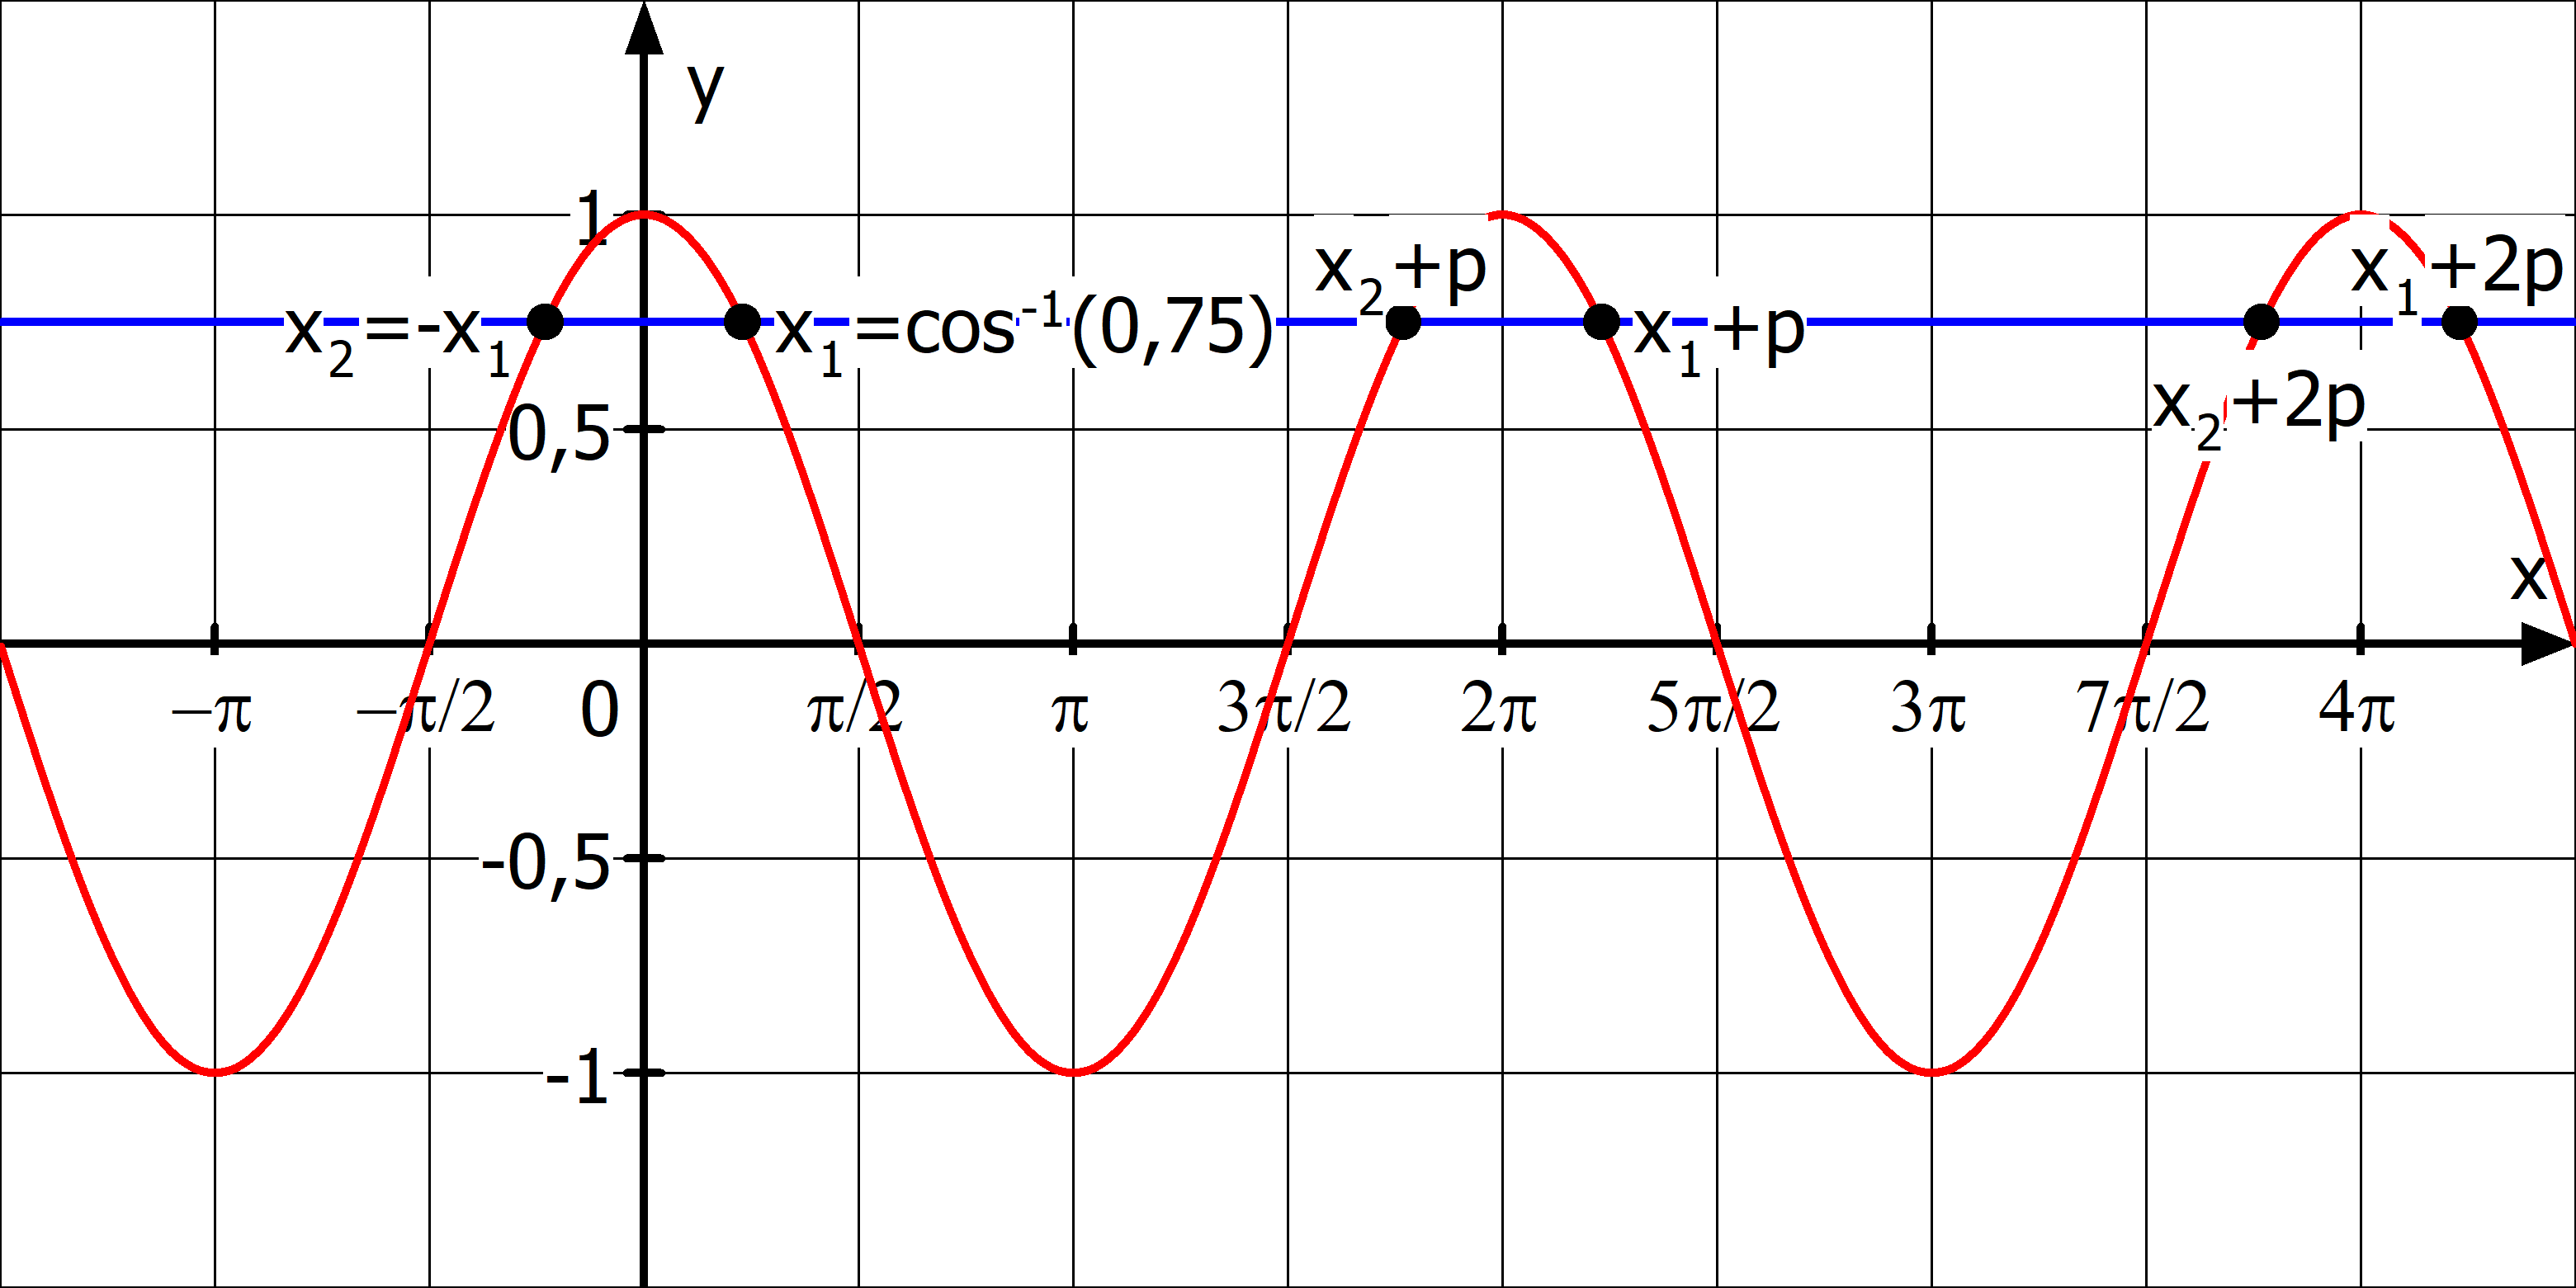
\includegraphics[width=.95\linewidth]{\trigonometrie/pics/Gleichungen_cos.png}\\
\end{minipage}
\begin{enumerate}
	\item Gleichung zu \(\cos(x)=r\) umformen
	\begin{align*}
		\textcolor{loes}{2\cos(x)}&\textcolor{loes}{=1,5\ \vert :2}\\
		\textcolor{loes}{\cos(x)}&\textcolor{loes}{=0,75}\\
	\end{align*}
	\item Erste Lösung mit Hilfe der Umkehrfunktion \(\cos^{-1}\) bestimmen
	\begin{align*}
		\textcolor{loes}{\cos(x)}&\textcolor{loes}{=0,75\ \vert \cos^{-1}}\\
		\textcolor{loes}{x_1}&\textcolor{loes}{=\cos^{-1}(0,75)}\\		
	\end{align*}
	\textcolor{loes}{ACHTUNG: In \(\cos^{-1}(y)\) dürfen nur Werte \(-1\leq y \leq1\) eingesetzt werden, da \(\cos(x)\) nur \(y\)-Werte zwischen -1 und 1 annimmt.}
	\item Zweite Lösung aus Symmetrie bestimmen\\
	\textcolor{loes}{Da das Schaubild von \(\cos(x)\) achsensymmetrisch zur \(y\)-Achse ist, ist eine zweite Lösung durch \(x_2=-x_1=-\cos^{-1}(0,75)\) gegeben.}\\
	\item Alle Lösungen bestimmen\\
	\textcolor{loes}{Beide Lösungen wiederholen sich im Abstand der Periode, die durch \(p=2\pi\) gegeben ist:\\
		\(x_k=x_1+2\pi k=\cos^{-1}(0,75)+2\pi k\text{ oder } x_k=x_2+2\pi k=-\cos^{-1}(0,75)+2\pi k,\ k\in \Z\)} 
\end{enumerate}
\newpage
Das gleiche Vorgehen kann zum Lösen von Gleichungen der Form \(\sin(x)=r\) verwendet werden: \(4\sin(x)=2\)\\
\begin{minipage}{\textwidth}
	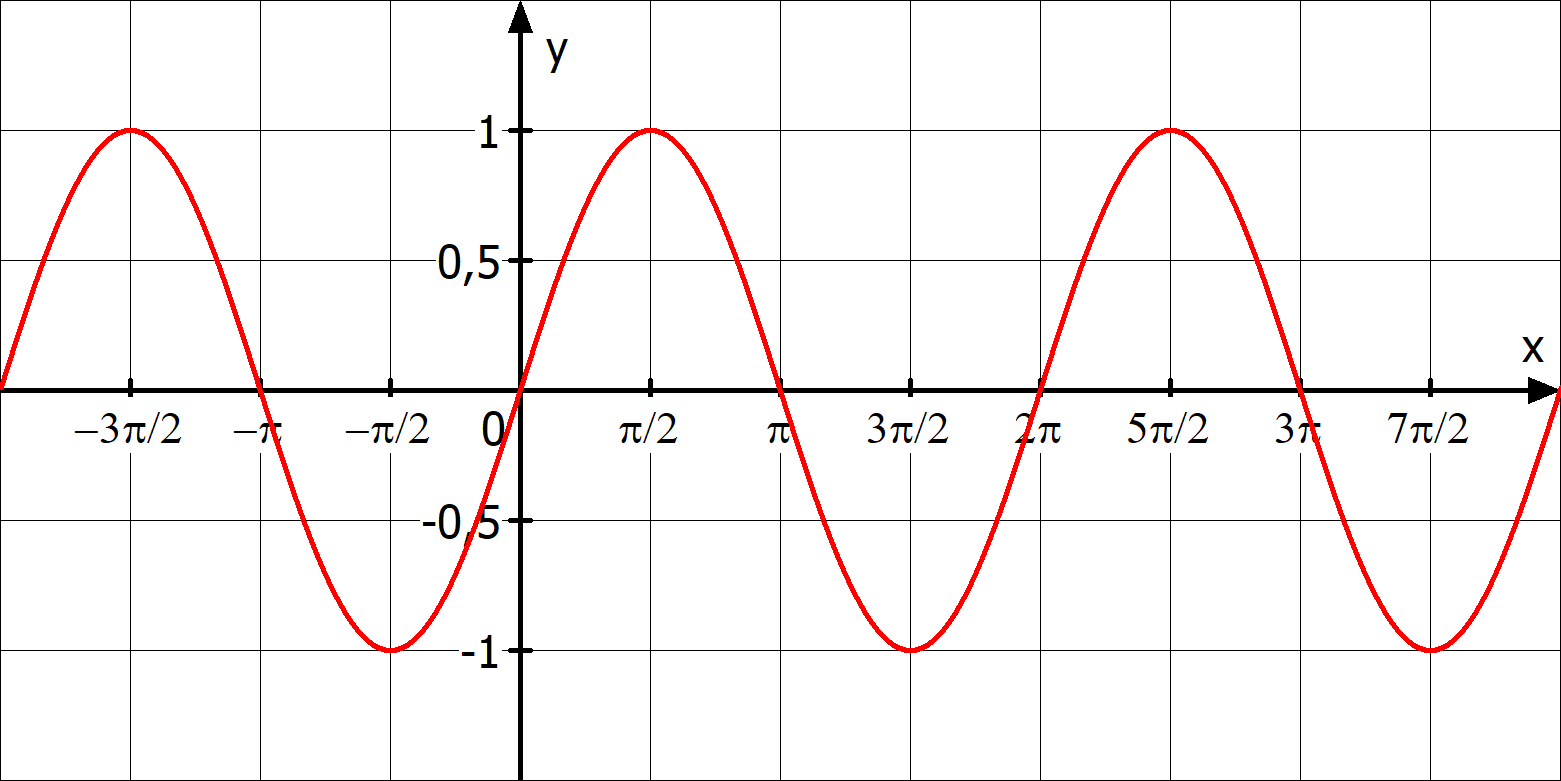
\includegraphics[width=.95\linewidth]{\trigonometrie/pics/Gleichungen_sin.png}\\
\end{minipage}
\begin{enumerate}
	\item Gleichung zu \(\sin(x)=r\) umformen
	\begin{align*}
		\textcolor{loes}{4\sin(x)}&\textcolor{loes}{=2\ \vert :4}\\
		\textcolor{loes}{\sin(x)}&\textcolor{loes}{=0,5}\\
	\end{align*}
	\item Erste Lösung mit Hilfe der Umkehrfunktion \(\sin^{-1}\) bestimmen
	\begin{align*}
		\textcolor{loes}{\sin(x)}&\textcolor{loes}{=0,5\ \vert \sin^{-1}}\\
		\textcolor{loes}{x_1}&\textcolor{loes}{=\sin^{-1}(0,5)}\\
		\textcolor{loes}{x_1}&\textcolor{loes}{=\frac{\pi}{6}}\\		
	\end{align*}
	\textcolor{loes}{ACHTUNG: Für \(\sin^{-1}(y)\) gelten die gleichen Einschränkungen wie für \(\cos^{-1}(y)\), es dürfen nur Werte \(-1\leq y \leq1\) eingesetzt werden, da auch \(\sin(x)\) nur \(y\)-Werte zwischen -1 und 1 annimmt.}
	\item Zweite Lösung aus Symmetrie bestimmen\\
	\textcolor{loes}{Da das Schaubild von \(\sin(x)\) achsensymmetrisch zur Achse \(x=\frac{\pi}{2}\) ist, ist eine zweite Lösung durch \(x_2=\pi-x_1=\pi-\frac{\pi}{6}=\frac{5\pi}{6}\) gegeben.}\\
	\item Alle Lösungen bestimmen\\
	\textcolor{loes}{Beide Lösungen wiederholen sich im Abstand der Periode, die durch \(p=2\pi\) gegeben ist:\\
		\(x_k=x_1+2\pi k=\frac{\pi}{6}+2\pi k\text{ oder } x_k=x_2+2\pi k=\frac{5\pi}{6}+2\pi k,\ k\in \Z\)} 
\end{enumerate}

\newpage
\begin{Exercise}[title={\raggedright\normalfont Bestimme jeweils alle Lösungen:}, label=sincosGleichungenA1]
	\begin{enumerate}[label=\alph*)]
		\item \(\sin(x)=-\frac{1}{2}\)
		\item \(-2\sin(x)=\sqrt{2}\)
		\item \(\cos(x)=\frac{\sqrt{3}}{2}\)
		\item \(3\cos(x)=-2\)
		\item \(\sin(x)=2\)
		\item \(2\cos(x)+1=3\)
		\item \(\sin(x)=0\)
		\item \(-\cos(x)-2=-1,7\)
		\item \(5\sin(x)=1\)
		\item \(3\sin(x)=-1\)
		\item \(4\cos(x)=-2\sqrt{2}\)
		\item \(\frac{2}{3}\cos(x)=\frac{1}{6}\)
		\item \(-\sin(x)-1,5=-1,1\)
		\item \(0,5\cos(x)=0,6\)
		\item \(2\cos(x)+2=\frac{3}{2}\)
		\item \(-\frac{7}{5}\cos(x)-\frac{1}{5}=\frac{1}{10}\)
		\item \(-5\sin(x)-2=2\)
		\item \(\sin(x)+3=-3,1\)
		\item \(-2\cos(x)-\frac{1}{2}=-1\)
		\item \(-4\sin(x)+6=-9\)
		\item \(\cos(x)-10=-10,8\)
		\item \(-5\sin(x)+10=-10\)
		\item \(-\frac{7}{8}\cos(x)+\frac{1}{4}=\frac{3}{8}\)
		\item \(-\frac{3}{2}\sin(x)-\frac{5}{2}=-\frac{20}{9}\)
		\item \(\frac{4}{3}\sin(x)+\frac{8}{3}=\frac{5}{3}\)
		\item \(\frac{8}{3}\cos(x)-1=0\)
	\end{enumerate}
\end{Exercise}

%%%%%%%%%%%%%%%%%%%%%%%%%%%%%%%%%%%%%%%%%
\begin{Answer}[ref=sincosGleichungenA1]
	\begin{enumerate}[label=\alph*)]
		\item \(x_k=-\frac{\pi}{6} +2\pi k\text{ oder }x_k=\frac{7\pi}{6} +2\pi k,\ k\in\Z\)
		\item \(x_k=-\frac{\pi}{4} +2\pi k\text{ oder }x_k=\frac{5\pi}{4} +2\pi k,\ k\in\Z\)
		\item \(x_k=\pm \frac{\pi}{6} +2\pi k,\ k\in\Z\)
		\item \(x_k=\pm \arccoss{-\frac{2}{3}} +2\pi k\approx \pm 2,30 +2\pi k,\ k\in\Z\)	
		\item keine Lösungen
		\item \(x_k=2\pi k,\ k\in\Z\)
		\item \(x_k=2\pi k\text{ oder }x_k=\pi +2\pi k=\pi k,\ k\in\Z\)
		\item \(x_k=\pm \arccoss{-0,3} +2\pi k\approx \pm 1,88 +2\pi k,\ k\in\Z\)
		\item \(x_k=\arcsinn{\frac{1}{5}} +2\pi k\approx 0,20+2\pi k\text{ oder }x_k=\pi-\arcsinn{\frac{1}{5}} +2\pi k\approx 2,94+2\pi k,\ k\in\Z\)
		\item \(x_k=\arcsinn{-\frac{1}{3}} +2\pi k\approx -0,34+2\pi k\text{ oder }x_k=\pi-\arcsinn{-\frac{1}{3}} +2\pi k\approx 3,48+2\pi k,\ k\in\Z\)
		\item \(x_k=\pm \frac{3\pi}{4} +2\pi k,\ k\in\Z\)
		\item \(x_k=\pm \arccoss{\frac{1}{4}} +2\pi k\approx \pm 1,32 +2\pi k,\ k\in\Z\)
		\item \(x_k=\arcsinn{-\frac{2}{5}} +2\pi k\approx -0,41+2\pi k\text{ oder }x_k=\pi-\arcsinn{-\frac{2}{5}} +2\pi k\approx 3,55+2\pi k,\ k\in\Z\)
		\item keine Lösungen
		\item \(x_k=\pm \arccoss{-\frac{1}{4}} +2\pi k\approx \pm 1,82 +2\pi k,\ k\in\Z\)
		\item \(x_k=\pm \arccoss{-\frac{3}{14}} +2\pi k\approx \pm 1,79 +2\pi k,\ k\in\Z\)
		\item \(x_k=\arcsinn{-\frac{4}{5}} +2\pi k\approx -0,93+2\pi k\text{ oder }x_k=\pi-\arcsinn{-\frac{4}{5}} +2\pi k\approx 4,07+2\pi k,\ k\in\Z\)
		\item \(x_k=\arcsinn{-0,1} +2\pi k\approx -0,10+2\pi k\text{ oder }x_k=\pi-\arcsinn{-0,1} +2\pi k\approx 3,24+2\pi k,\ k\in\Z\)
		\item \(x_k=\pm \arccoss{\frac{1}{4}} +2\pi k\approx \pm 1,32 +2\pi k,\ k\in\Z\)
		\item keine Lösungen
		\item \(x_k=\pm \arccoss{-0,8} +2\pi k\approx \pm 2,50 +2\pi k,\ k\in\Z\)
		\item keine Lösungen
		\item \(x_k=\pm \arccoss{-\frac{1}{7}} +2\pi k\approx \pm 1,71 +2\pi k,\ k\in\Z\)
		\item \(x_k=\arcsinn{-\frac{5}{27}} +2\pi k\approx -0,19+2\pi k\text{ oder }x_k=\pi-\arcsinn{-\frac{5}{27}} +2\pi k\approx 3,33+2\pi k,\ k\in\Z\)
		\item \(x_k=\arcsinn{-\frac{3}{4}} +2\pi k\approx -0,85+2\pi k\text{ oder }x_k=\pi-\arcsinn{-\frac{3}{4}} +2\pi k\approx 3,99+2\pi k,\ k\in\Z\)
		\item \(x_k=\pm \arccoss{\frac{3}{8}} +2\pi k\approx \pm 1,19 +2\pi k,\ k\in\Z\)
	\end{enumerate}
\end{Answer}